\documentclass[12pt,a4paper]{report}
\fontfamily{times_new_roman}
\selectfont
\usepackage{amsmath}
\usepackage{graphicx}

\usepackage[colorlinks=true,linkcolor=red]{hyperref}%%%%%%

\usepackage[left=1in,right=1in,top=1in,bottom=1in]{geometry}% to set margins

\begin{document}
\renewcommand{\baselinestretch}{1.15}
\begin{center}

\noindent \textbf{A Report  on}

\noindent \textbf{ADVANCED SAFETY HELMET FOR WORKERS }

\noindent \textbf{}
\end{center}
\noindent 
\begin{center}
\noindent{SUBMITTED TO THE SAVITRIBAI PHULE PUNE UNIVERSITY, PUNE}
\end{center}

\begin{center}
\begin{figure}[htp]
    \centering
    \includegraphics[width=4cm]{LOGO1.png}
\end{figure}
\end{center}

\begin{center}
\noindent IN THE \textbf{PARTIAL FULFILLMENT OF PROJECT PART-II} OF THE REQUIREMENTS FOR THE AWARD OF THE DEGREE OF
\end{center}
\begin{center}
    \noindent \textbf{BACHELOR OF ELECTRONICS\&TELECOMMUNICATION ENGINEERING }

\noindent by

\begin{table}[h]
\centering
\large{}
\begin{tabular}{ll}
\textbf{Mrunal Jadhav}    & \textbf{(BEENTC25)} \\
\textbf{Niraj Mistri} & \textbf{(BEENTC37)} \\
\textbf{Akansha Pole}   & \textbf{(BEENTC53)} 
\end{tabular}
\end{table}

\vspace{0.1cm}
\normalsize{UNDER THE GUIDANCE OF}\\
\large{\textbf{Prof. Arti Tekade
\end{center}
}}
\begin{center}
\noindent \textbf{Department of Electronics and Telecommunication Engineering Pimpri Chinchwad College of Engineering and Research,Ravet,}

\noindent \textbf{Pune-412101}
\end{center}
\begin{center}
\noindent \textbf{ACADEMIC YEAR:2021-22}
\end{center}
\noindent 
\newpage
\noindent 
\begin{center}
    
\item \subparagraph{PIMPRI CHINCHWAD EDUCATION TRUST'S}
\end{center}
\begin{center}
\newline\textbf{Pimpri Chinchwad College of Engineering and Research, Pune-412101}
\end{center}

\begin{center}
\begin{figure}[htp]
    \centering
    \includegraphics[width=4cm]{PCCOERLOGO.png}
\end{figure}    
\end{center}

\begin{center}
    
\noindent \textbf{CERTIFICATE}
\end{center}
\begin{center}
\noindent This is certified that the project phase II report entitled

\noindent ``\textbf{Advanced Safety Helmet for Workers} '',

\noindent               Submitted by
\end{center}
\begin{center}

\normalsize{}
\begin{tabular}{ll}
\textbf{Mrunal Jadhav}    & \textbf{(BEENTC25)} \\
\textbf{Niraj Mistri} & \textbf{(BEENTC37)} \\
\textbf{Akansha Pole}   & \textbf{(BEENTC53)} 
\end{tabular}
\end{center}
\noindent is a bonafide work carried out by them under the supervision of \textbf{Prof. Arti Tekade }and it is approved for the partial fulfillment of the Project Phase II of the requirement of Savitribai Phule Pune University, Pune for the award of the degree of Bachelor of Engineering (Electronics \&Telecommunication).The Dissertation work has not been earlier submitted to any other institute or university for the award of degree.
\newline
\newline
\noindent 
% Please add the following required packages to your document preamble:
% \usepackage[normalem]{ulem}
% \useunder{\uline}{\ul}{}
\begin{table}[h]
\centering
\begin{tabular}{ccllllllcllc}
Prof. Arti Tekade  &           &  &  &  &  &  &  &           &  &  & Prof. Kishore Bhangale        \\
\textbf{Project Guide}      & \textbf{} &  &  &  &  &  &  & \textbf{} &  &  & \textbf{Project Coordinator} \\
                            &           &  &  &  &  &  &  &           &  &  &                              \\
                            &           &  &  &  &  &  &  &           &  &  &                              \\
                            &           &  &  &  &  &  &  &           &  &  &                              \\
                            &           &  &  &  &  &  &  &           &  &  &                              \\
Prof. Dr. Rahul G.  Mapari  &           &  &  &  &  &  &  &           &  &  & Prof. Dr. H. U. Tiwari       \\
\textbf{Head of Department} & \textbf{} &  &  &  &  &  &  & \textbf{} &  &  & \textbf{Principal}          
\end{tabular}
\end{table}
\newpage
%%Acknowledgement

\chapter*{Acknowledgement\markboth{Acknowledgement}{Acknowledgement}}
\noindent
We are greatly indebted to Head of Electronics \& Telecommunication Engineering and Project Guide \textbf{Prof.Arti Tekade }for her able guidance throughout the course of this work. It has been anal together different experience to work with her and we would like to thank her for her help, suggestions and numerous discussions.

\noindent 

We are heartily thankful to Prof.\textbf{ Dr.Harish.U.Tiwari  }(Principal,  Pimpri  Chinchwad College of Engineering \& Research,Ravet)for providing research environment; also for his kind inspiration.



We are gladly taking this opportunity to thank Head of Electronics Telecommunication Engineering \textbf{Prof. Dr.Rahul Mapari }and project Coordinator \textbf{Prof.Kishor Bhangale  }for their valuable guidance and providing facility during progress of seminar. We would like to express our sincere thanks to \textbf{Prof.Arti Tekade for} providing continuous support to complete our project. Her knowledge helped us to achieve desired outcomes. Last but not least we are also thankful to all those who help directly or indirectly to develop this Project work and complete it successfully. With Deep Reverence,

\noindent 
\begin{table}[h]
\large{}
\begin{tabular}{lllllllllllllllllllllllllllllll}
 &  &  &  &  &  &  &  &  &  &  &  &  &  &  &  &  &  &  &  &  &  &  &    \textbf{Mrunal Jadhav}    \\
 &  &  &  &  &  &  &  &  &  &  &  &  &  &  &  &  &  &  &  &  &  &  &     \textbf{Niraj Mistri} \\
 &  &  &  &  &  &  &  &  &  &  &  &  &  &  &  &  &  &  &  &  &  &  &   \textbf{Akansha Pole}  
\end{tabular}
\end{table}
\paragraph{}\textbf{Date:}
\paragraph{}\textbf{Place:}
\newpage

\tableofcontents
\listoffigures
\listoftables

\noindent
\newpage
%abstract
\begin{abstract}

%%Type abstract here instead of below content


A novel design of flexible solution of underground mine workers' safety with advanced technology using temperature sensor, heart rate sensor, smoke detection sensor is presented here.

Mining is world's most dangerous professions. In some nations, underground miners lack safety and social protection, be left to fend for themselves if injured. Additionally, there are adverse societal repercussions, including displacement and loss of livelihood. Mining has the greatest fatality rate of any industry. The most workplace fatalities poisoning, and electrocution.In the system temperature sensor, heartbeat sensor, smoke sensor , buzzer, WIFI module is used. Sensors will read the values and send it to the controller . If the conditions of environment changes like if smoke at the workers end increases system send alert. Hence our system is helpful for the worker.
\newline
\noindent
\noindent    Keywords---\textbf{ }Internet of Things (IOT), Wi-Fi, Cloud Think Speak, Python 8.
\end{abstract}
\noindent 

\noindent 

\noindent 

\noindent 
\newpage

%%%CHAPTER 1
\chapter{Introduction}
\hspace{6pt}
%\large{Paragraph 1 of introduction . }
\section{Introduction}

\noindent The internet is one of the greatest human inventions in the world. It has   changed and improved the means of people; also, it has been  evolving each  and every day. In this innovation, concept called the 'Internet of Things' (IoT) helps in making devices smarter with interactive computing and wireless's connected embedded devices. In whatever form of construction, worker safety should always be a primary priority. Underground mining operations are a high-risk achieve in terms of worker safety and health. The various procedures used to  harvest various minerals are main dangerous problem for these hazards. The deeper the mine, the higher the risk occurs. These issues about safety are especially severe in the coal business. As a result, worker safety should be a major priority in any type of mining, whether coal or other minerals.[1] 

\noindent Underground coal mining is more threatening than open pit mining due to ventilation concerns and the possibility of collapse. The use of heavy machinery and excavation procedures, are the reason behind safety dangers in all types of mining. Modern mines routinely follow a wide range of safety protocols, worker education and training, and health and safety requirements, resulting in considerable importance and improvements in both opencast and underground mining.[2]

\noindent Safety is the most vital part of any type of industry. In the mining industry safety and security is a fundamental aspect of all. To avoid any type of harmful accidents mining industry follows some basic precautions rules. 

\noindent Still accidents take place in underground mines due to rise in temperature, increased water level, and methane gas leakage. Here we provide safety to worker with the help of advanced safety helmet.

\noindent When worker is in danger the sensors present in the helmet makes the buzzer on  according to the conditions given in code and inform security. To enhance safety in underground mines, a well-founded communication system must be established between workers in underground mines and fixed ground mine system[3]

\noindent The communication network must not be interrupted at any moment and at any condition. A cost-effective  wireless mine supervising system with early-warning intelligence is proposed in this project. Worker status can be monitor over IOT and the data is saved in the cloud.

\noindent Modern mines often implement several safety procedures, education and training of workers, health and safety standards, which lead to significant changes and improvements in opencast and underground mining. Coal has always been the primary resource of energy in India, which has a large amount of contribution to the rapid industrial development of the country.[4]

\noindent The implementation of heavy machinery and the methods performed during excavations result into safety risks in all types of mining . Coal has always been the primary resource of energy in India, which has significantly contributed to the rapid industrial development of the country. 

\noindent About 70\% of the power generation is dependent on it therefore, the importance of coal in energy sector is irreplaceable. But the production brings with it the other by products, which proves to be a potential threat to the environment and the people associated with it. 

\noindent In consideration of that the present work is a sincere attempt in  Analyzing the graveness and designing a real time monitoring system of detection by using the Wi-Fi technology, also by saving the data in cloud .

\noindent Thing Speak is an IoT analytics platform service that allows you to aggregate, visualize and analyze live data streams in the cloud. Thing Speak provides instant visualizations of data posted by your devices to Thing Speak.[5]

\noindent 


\section{ Research background}

\noindent Mining is one of the most dangerous trades all over the world. In some countries, underground miners lack safety, social guarantees and in case of injury may be left to cope without assistance. There are negative social impacts as well as displacement and lost livelihoods. The mining industry has the highest incidence of occupational deaths among all duties. 

\noindent Common causes of occupational deaths include rock falls, fires, explosions, methane intoxication, and electrocution. There are many case studies behind underground mines, a recent case study in China reveals that underground mining in China is the world's deadliest industry. To overcome all these disasters, we have developed a better communication technology which has to be employed for an intelligent sensing and warning system.[6]

\noindent Safety is the most vital part of any type of industry. In the mining industry safety and security is a fundamental aspect of all. To avoid any types of accidents mining industry follows some basic precautions. The entire system is implemented using Raspberry-Pi. Mine ventilation system can help in eliminating high risk atmosphere. 

\noindent Integrating ventilation monitoring system enables mine to intelligently make ventilation changes based on the extensive data, the monitoring system provides. Mine ventilation system can help in eliminating high risk atmosphere. Primitive techniques to monitor the mining atmosphere can be traced back to the use of canaries and other animals to alert miners, when the atmosphere becomes toxic.[7]

\noindent 


\section{ Problem Statement}

\noindent          ``The main aim of this project is to developed IOT Based Tracking and working smart safety helmets''

\noindent 


\susection{ Objectives of the Study}

\noindent The objectives of the proposed works are mentioned as follow 

\begin{enumerate}
\item  To avoid the conditions of environment changes.

\item  To maintain security is a fundamental aspect of all.

\item  To avoid accidents of workers working in mining industries. 

\item  Detection of the poisonous gases. 

\item  Alerting the miners whenever the helmet is removed.

\item  Assuring miners' safety in case of mining accidents that occurs due to increase in temperature, Heart rate, smoke detected.
\end{enumerate}

\noindent 


\section{ Scope of the Study}

\noindent The utilization of a sewage monitoring system sets in place a useful approach to remind individuals or facilities employing these workers, to evacuate areas when ppm levels of certain gases goes higher than recommended. This saves lives of the employees working in harmful environments and saves them from hazards.

\noindent Organizations often employ septic tanks and chemical treatment of sewage sites in industries prior to sending in manual workers on site, however no system is in place to check on hazardous levels. A smart system is defined as  an embedded system, that can process sensor data and assure a wireless communication to the server. Different systems have been proposed earlier by scientists researching the environmental pollution and air hazards due to industrial sewage.

\noindent For example, IoT might be used to address the air pollution problem, as proposed in pollution to check Ground-level ozone. That gives rise to respiratory diseases such as Sulphur dioxide, nitrogen oxides or airborne particles caused by emission of polluting gases from vehicles that degrade air quality. In survey a design is proposed that brings in Wireless Sensor Networks (WSN) for air pollution monitoring system, called Wireless Sensor Network Air Pollution Monitoring System (WAPMS). In this example they have designed an intelligent residential security alarm and remote-control system on the basis of single chip computer to check on toxic gas leakage in homes. The Internet of Things (IoT) is broadly being perceived by analysts as a standout amongst the most modern advancements with the plan to significantly change livelihood, security and security and addresses real effects inside the general public. This breakthrough in technology can be used in collaboration with sensors, and a smart system is designed for industrial purposes.[8]

\noindent 


\section{ Overview of Proposed System}

\noindent                          In this project  implemented an ultimate protective helmet that comes with many sensors for various detection and analysis.The dangerous gases are sensed using gas sensors. Every time the poisonous gas is sensed the control valve gets opened for providing oxygen companion.

\noindent                              In this project the raspberry pi is the major controller. System is able to monitor the health conditions of the worker as well as surrounding conditions. Also, if the worker health disturbed system will send the alert message.

\noindent      In the system temperature sensor, heartbeat sensor, smoke sensor , buzzer, WIFI module is used. Sensors will read the values and send it to the controller . If the conditions of environment changes like if smoke at the workers end increases system send alert. Hence our system is helpful for the worker.

\begin{figure}[htp]
    \centering
    \includegraphics[width=18cm]{block diagram.png}
    \caption{Block Diagram}
\end{figure}

\noindent 
\newpage
\section{Organization of the Report}

\noindent The project report is organized as follow:

\noindent Chapter 1 describes the introduction of project, it contains background, need and motivation, problem statement, objectives, scope and significance of project.

\noindent Chapter 2 provides information regarding the literature survey and gap identification from the survey 

\noindent Chapter 3 describes the methodology used with the help of block diagram and flowchart 

\noindent Chapter4 describes the hardware and software specifications 

\noindent Chapter 5 gives us the experimental results of the project 

\noindent Chapter 6 use of project like applications, advantages and disadvantages 

\noindent Chapter 7 conclusion and future e scope as well as reference papers

\noindent \textbf{}
\newpage
%CHAPT 2
\chapter{Literature Review}

\noindent During the literature survey  came across different papers to know how our project is related to the previous work done by others on this topic. Thus, understood the basic methodology.


\section{ Literature Review}

\noindent Primitive procedures of monitoring a mine's air can be followed back to the utilization of canaries and different creatures to ready diggers when the climate gets to be lethal. Inappropriate ventilation monitoring systems empowers a mine to insightfully roll out ventilation improvements in view of the far-reaching information given by the monitoring systems. Sudden changes in the ventilation system are identified by the monitoring system, permitting quick move to be made. New and creating correspondence and following systems can be used to monitor mines more proficiently and transfer the information to the surface.

\noindent The progression of technology has allowed mine monitoring techniques to become more sophisticated, yet explosions in underground coal mines still occur. The safety issues of coal mines have gradually turned into a major concern for the society and nation.

\noindent  The occurrence of disasters in coal mines is mainly due to the harsh environment and variability of working conditions.So, it makes the implementation of mine monitoring systems essential for the safety purpose. Wired network systems used to be a trend for traditional coal mines, which have really played a significant role in safely production in coal mines.[9][10]


\section{ Finding from Literature Survey}

\paragraph\noindent  Asthana et al. [11] This project aims at providing smart solutions to monitor poisonous sewage gases and works on a system of live sewage level detection and monitoring. Whenever, a certain threshold is crossed, an alert is sent to the observer who is examining the conditions from a remote location. The information is then forwarded along with different gas ppm values indicating whether it is safe for the worker to clean or work in that environment or not. The remotely placed IoT monitoring equipment and IoT platform are integrated to create proposed system.

\noindent This requires calibration of gas sensors for industrial purposes and determining the correct threshold levels for septic plants and facilities. The hardware is designed such that it shall send a prior alert to the sewage worker to ensure their safety, if damaging gaseous constituents increase in concentration over time. Various types of sensors are utilized to monitor parameters present in sewage like gas, temperature etc. When the threshold value is lesser than the sensed values, this system alerts the sewage worker/cleaner by sending SMS and call alerts by analyzing concentrations of different toxic gases and graphing out their results for real-time monitoring thereby aiding in protection from hazardous diseases and hence serves a social cause as well. 

\noindent In the proposed system, sample values for sensors have been recorded and plotted on Thing Speak analysis tool. Carbon monoxide and methane sensors charted values up-to 2.3 and 60 ppm respectively, and this breached threshold and GSM module was utilized for sending alert to mobile number fed in the code.

\noindent 
\paragraph\noindent Emmanuel Freeman1et al.[12] Detecting water leakage and reporting the leakage timely is one of the challenges faced by water distributing companies in developing nations. This paper employs a nature-inspired search method for optimal location search to water leakage sources for Ghana Water and Sewage Services Company. The nature-inspired method aid in mapping IoT-edge computing devices used by the water and sewage workers, especially in the cities and urban areas, to find and locate leaked pipelines. Once, a water and sewage worker receive a trigger from any location that there are leakages, the algorithm generates the location data which automatically processes the distance, geographic location, and direction. 

\noindent In this paper, a nature-inspired algorithm based on the behavior of a Kestrel bird was used as the mapping function. The developed algorithm was tested and evaluated using pre-defined and random locations based on their latitudes and longitudinal data. The proposed algorithm was evaluated against BAT algorithm. Findings from the data indicated that the proposed KSA used as mapping function, was successful in providing the optimal distance after receiving water leakage geographic location data from IoT edge computing devices.

\noindent 

\paragraph\noindent Haswan et al.[13] Drainage is the system or process by which water, sewage or other liquids are drained from a place and to maintain the proper function of drainage, its condition should be monitored regularly. But manually it is very difficult to monitor all area where a human cannot reach. 

\noindent This influences the blockage of underground pipes and overflows of water cause the health problem. To mitigate all these issues here we are developed and implemented the system using wireless sensor network. It consisting of small devices used to collect data. These sensing devices are called node. The proposed system is low cost, less maintenance, long life and web-based real time system, which update the municipal officer by text message when any manhole crosses the threshold value. This system directly impacts on the health issues of citizens and worker who cleans the underground drainage.

\noindent  It also avoids spreading of infection due to mosquitoes and gives clean and healthy environment as well as controls the diseases such as malaria, dengue, diarrhea, etc. The system reduces the accident caused by an exposed manhole.

\noindent 

\paragraph\noindent Tian et al. [14] Sewage Treatment is becoming more important by the development of the worldwide industry. But bad environment of sewage farm brings wireless system a series of problem. To solve the problem, a measurement and control system by virtue of wireless Mesh network is designed in this paper. In this control system, we design the sensor node based on AT89C2051and nRF2401, which can collect needed locale information to complete sewage treatment and monitor the power of the machine to avoid accident under the condition of without cable.

\noindent  The experimental results show that this measurement and control system can realize the automation process of sewage treatment and has good system performance, it also provides the worker convenience monitoring.

\noindent 

\paragraph\noindent Malakahmad et al. [15] Sewage treatment plant (STP) operators are exposed to variety of hazard during wastewater processing. The aim of this study is to identify and manage these hazards, particularly in a local STP in Malaysia, through Occupational Health and Safety Management System (OSHMS). 

\noindent Initially, reported hazards data were collected via review of literatures, questionnaire distribution and interview with experts. Then, the most risky hazards based on conditions of selected STP were identified. Subsequently, the hazards were ranked based on severity and likelihood. Results show exposure to excessive noise, skin irritation and slip and fall are the main concerns of workers in the site. Therefore, noise mitigation was done using sound absorbers.

\noindent  It was indicated that the level of existing noise (94.2 dB) was reduced to 92.1 dB and 90.6 dB by application of carpet and cardboard, respectively. Skin irritation risk is suggested to be mitigated by installation of auto-cleaner, self-cleaning bar screen and scraper blades at the site. 

\noindent In addition, cordoning off areas while cleaning is in progress and provision of ramps at cleaning area around the clarifier are found to be the appropriate solutions for slip and fall risk at the site.

\noindent 

\paragraph\noindent Priya et al. [16] Textile processing units largely employ azo dyes which are derivatives of benzene. Toxic sewage discharged from textile industries contains azo dyes. They affect soil fertility, water resources, marine organisms and the ecosystem. Benzidine is responsible for skin irritation and also increases the toxicity in blood and bone marrow which affects the production of blood cells and hence leads to anemia. 

\noindent Exposure to these benzidine dyes can induce hemolytic anemia which leads to deformation of Red Blood Cells (RBCs). In this work, an automated detection of toxicity is proposed to alert the workers prior to the critical stages of cancer. The proposed system consists of a portable unit where the blood samples are analyzed and the toxic status of the dye factory workers can be transmitted from the local health center to the nearby hospital. 

\noindent Microscopic images of the smeared blood samples are acquired using the digital microscope. These RBC images of normal and abnormal are segmented using Laplacian of Gaussian (LoG) segmentation. Geometric shape-based features are extracted from the segmented images. Significant geometric features are chosen by conducting student's `t' test. 

\noindent It is observed from the results that these significant geometric features show discrimination between the normal and abnormal RBCs. This early detection of toxicity can help workers in the site to take immediate medication which could reduce the probability of adversity in their health condition.

\noindent 

\paragraph\noindent Priyanka et al.[17] Internet of things (IoT) remains one of the most electrifying and fast burgeoning fields. It permits most of the things like any objects are controlled with very less manpower and we can control things anywhere and anytime by using network. In this paper that going to be constructing that the ``Detection of Blockage in Manhole Using IoT''. 

\noindent Detecting a struck in the manhole pipe, due to blockage of sludge in a pipe. Here by using detecting the length of the pipe using ultrasonic sensor till where the sludge struck with the help of capturing image of sludge to aware of, due to gloominess inside a manhole by provide a luminescence, which helps to capture picture of particular sludge. And with the help of developing an application to control the device, by using that application data access can be done (captured picture) using a cloud. 

\noindent In traditional method, sewers have to do cleaning in all the cities (areas). In gutters, workers stand in the waste, which reaches chest level and with the help of long wooden sticks and broomsticks they clear blockage. 

\noindent In some area's workers crawl into a sewage, without wearing any protective gear. And those workers are treated very badly by the society. Thus, sewers need to work a lot to clear blockage. But now by using this technique it will be very much easier to reduce a man power and also incremental steps can be added further.

\noindent 

\paragraph\noindent Umapathi et al. [18] Maintenance of sewage system is a cumbersome task which has to be carried out in regular basis since it is inevitable. Domestic practices will produce some organic waste like leftover food, wet waste etc.which are released into drains. These wastes will release some of the hazardous gases like CH4, CO and H2S. The paper implements an idea of detecting sewage gases which are harmful, hence prevents the people working in sewage systems from gas poisoning.

\noindent  The developed system is aimed to alert the sewage workers by using an Arduino Mega, gas sensors and GSM Module. The system monitors sewage gases continuously and when the content of hazardous gas hits the set threshold value the Arduino sends an SMS alert to the registered number.

\noindent  For the people present nearby the values are displayed on LCD display. The system also has an ultrasonic sensor to measure the depth of sewer. The threshold and Alert message are set by coding the Arduino Mega.

\noindent 
\paragraph\noindent{ Pushpakumar et al. [19] The process of drainage monitoring and maintain plays a big role to keep the city neat and clean. This leads to an informal way of monitoring and cleaning the drainage manholes when it is blocked. The process of unblocking and cleaning process may lead to much human death because of the gas. Additionally, some of the time because of the absence of information the specialist may meet to a mishap as they have no clue about the state of the gas level in the seepage. This paper helps to solve the problem by a smart device with the help of the IoT. The MQ4 sensor and the single board computer raspberry pi 3 helps to detect the gas level with the LED display.} 

\noindent This system will help to identify the gas level inside the drainage manholes so that the worker can get some idea of entering into the manholes. It very helps workers and safety to them before getting down into the manholes and it will sense the level of the gas inside. Savvy framework will be checking if the blockage has happened in the middle of two sewer vents and furthermore it will detect different gas level which is hurtful to individuals, and furthermore a framework observing the water level then it will trigger an alert and it will offer data to the crisis division and wellbeing offices which will make specific move at time. 

\noindent The framework will ready to screen every one of these things in the continuous situation which will enable us to make a legitimate move of the specific issue in seepage frameworks.

\noindent 

\paragraph\noindent Kumar et al. [20] A large number of sanitation workers die every year due to erratic and lack of facilities available, and harmful toxic gases released while cleaning the sewage. Real time health monitoring systems for such workers will work in a sewage as a safety equipment. In our project, the device will monitor the pulse rate of the person using a Heartbeat sensor and the concentration of CH4with respect to atmospheric O2 and provide alert to the worker and exterior unit when parameters deviate from the safe range. 

\noindent This outcome will promptly alert the worker to stay safe and detect the toxic gases before any harm.

\noindent 

\noindent 
\newpage


\noindent \textbf{}

%CHAPT 3
\chapter{Proposed Methodolgy}
\hspace{7pt}


\noindent Modern mines often implement several safety procedures, education and training for workers, health and safety standards, which lead to substantial changes and improvements and safety level both in opencast and underground mining. The hazardous gases are detected using gas sensors. Whenever the poisonous gas is detected the solenoid valve gets opened for providing oxygen supplements.

\noindent In the project raspberry pi is the main controller . System is able to monitor the health conditions of the worker as well as surrounding conditions. Also, if the worker health disturbed system will send the alert message.

\noindent In the system temperature sensor, heartbeat sensor, smoke sensor , buzzer, WIFI module is used. Sensors will read the values and send it to the controller . If the conditions of environment changes like if smoke at the workers end increases system send alert. Hence our system is helpful for the worker.

\noindent In consideration of that the present work is a sincere attempt in  Analyzing the graveness and designing a real time monitoring system of detection by using the WIFI technology, also by saving the data in cloud.  These real-time ppm values are simultaneously updated to the cloud using Thing Speak IoT platform. The graphical representation of ppm values of these gases is plotted using the analytics tools in Thing Speak.

\noindent 


\section{ System Implementation/Block Diagram and Explanation}

\noindent 
\begin{figure}[htp]
    \centering
    \includegraphics[width=17cm]{ckt dia..png}
    \caption{Circuit Diagram}
\end{figure}

\noindent 


\noindent The hazardous gases are detected using gas sensors. Whenever the poisonous gas is detected the solenoid valve gets opened for providing oxygen supplements.

\noindent In the project raspberry pi is the main controller . System is able to monitor the health conditions of the worker as well as surrounding conditions. Also, if the worker health disturbed system will send the alert message. In the system temperature sensor, heartbeat sensor, smoke sensor , buzzer, WIFI module is used. Sensors will read the values and send it to the controller . If the conditions of environment changes like if smoke at the workers end increases system send alert. Hence our system is helpful for the worker.

\noindent In consideration of that the present work is a sincere attempt in  Analyzing the graveness and designing a real time monitoring system of detection by using the WIFI technology, also by saving the data in cloud. 

\noindent 

\noindent 

\noindent 

\noindent 



\noindent               

\noindent 


\section{ Design and Formulation}

\noindent 
{Raspberry Pi and Wi-Fi module are the primary components which make up this project model. Raspberry Pi enables it to read sensor data such as the ppm values collected from gas sensor . }

\noindent 
{Further, these real-time ppm values are simultaneously updated to the cloud using Thing Speak IoT platform. The graphical representation of ppm values of these gases is plotted using the analytics tools in Thing Speak.}

\noindent 
{ Finally, the status or an alert is sent to the mobile of the user when the values reach the threshold value using the GSM module. The data of the ppm values of the sensors can be stored and monitored by user so as to avoid any accident that might occur with the labor working at the sewage tanks and rescue them from health issues caused because of these harmful gases.}

\noindent 


\section{ Flow Chart and algorithm}

\noindent 


\noindent 


\noindent 

\noindent 

\noindent A flowchart is a picture of the separate steps of a process in sequential order. It is a generic tool that can be adapted for a wide variety of purposes, and can be used to describe various processes, such as a manufacturing process, an administrative or service process, or a project plan.

\noindent Above figure represents the algorithm of the whole project in an easier and simplest form. 

\noindent When the system starts it receives data from the workers unit future the received data parameters are displayed on the monitor display depending upon the environmental conditions the state of buzzer is decided the final data is send to the cloud think speak and is saved in the cloud.

\noindent 
\begin{figure}[htp]
    \includegraphics[width=18cm]{2022-05-22.png}
    \caption{Flow Chart}
\end{figure}


\newpage

\chapter{Results and Discussions}

\noindent In result we have taken some tests practically to know the exact values of Smoke sensor, temperatures sensor, Heartbeat Sensor. The result analysis of our project includes

\begin{enumerate}
\item  Sensing the gas leakage.

\item  Increase or decrease in temperature.

\item  Counting or detecting workers heart rate. 

\item  Transmission of data using Wi-Fi(THINKSPEAK).
\end{enumerate}

\noindent 


\section{ Hardware Setup}

\noindent{ Hardware Components and Specifications }
\noindent
\newline\textbf{1.Raspberry Pi 4 :-}
\begin{figure}[htp]
    \includegraphics[width=14cm]{raspbery pi.png}
    \caption{Raspberry Pi 4}
\end{figure}
\noindent 
\newline




\noindent \textbf{}

\noindent \textbf{}

\noindent \textbf{}

\noindent \textbf{}

\noindent \textbf{}

\noindent \textbf{}

\noindent \textbf{}

\noindent \textbf{}

\noindent \textbf{}

\noindent \textbf{}

\noindent \textbf{}

\noindent               

\noindent 

\noindent Raspberry Pi 4 Model B is the latest product in the popular Rasp berry Pi range of computers. It offers ground-breaking increases in processor speed, multimedia performance, memory, and connectivity compared to the prior-generation Raspberry Pi 3 Model B+, while retaining backwards compatibility and similar power consumption. For the end user, Raspberry Pi 4 Model B provides desktop performance comparable to entry-level x86 PC systems. This product's key features include a high-performance 64-bit quad-core processor, dual-display support at resolutions up to 4K via a pair of micro-HDMI ports, hardware video decode at up to 4Kp60, up to 4GB of RAM, dual-band 2.4/5.0 GHz wireless LAN, Bluetooth 5.0, Gigabit Ethernet, USB 3.0, and PoE capability (via a separate POE HAT add-on). The dual-band wireless LAN and Bluetooth have modular compliance certification, allowing the board to be designed into end products with significantly reduced compliance testing, improving both cost and time to market.

\noindent  Broadcom BCM2711, Quad core Cortex-A72 (ARM v8) 64-bit SoC @ 1.5GHz

\noindent  2GB, 4GB or 8GB LPDDR4-3200 SDRAM (depending on model)2.4 GHz and 5.0 GHz IEEE 802.11ac wireless, Bluetooth 5.0, BLE

\noindent  Gigabit Ethernet

\noindent  2 USB 3.0 ports; 2 USB 2.0 ports

\noindent  Raspberry Pi standard 40 pin GPIO header (fully backwards compatible with previous boards)

\noindent  2 $\mathrm{\times}$ micro- HDMI ports (up to 4kp60 supported)

\noindent  2-lane MIPI DSI display port 

\noindent  2-lane MIPI CSI camera port

\noindent  4-pole stereo audio and composite video port.

\noindent  H.265 (4kp60 decode), H264 (1080p60 decode, 1080p30 decode)

\noindent  Open GL ES 3.1, Vulkan 1.0

\noindent  Micro-SD Card slot for loading operating system and data storage.

\noindent  5V DC via USB-C connector (minimum 3A*)

\noindent  5V DC via GPIO header (minimum 3A*)

\noindent  Power over Ethernet (PoE) enabled (required separates PoE HAT)

\noindent  Operating Temperature:0-50 degrees C ambient

\noindent  A good quality 2.5A power supply can be used if downstream USB peripherals consume less than 500mA in total.

\noindent \textbf{}
\newpage
\begin{figure}[htp]
    \includegraphics[width=14cm]{memory slot .png}
    \caption{Raspberry Pi 4 Memory card Slot }
\end{figure}
\noindent

\noindent \textbf{}

\noindent The GPIO is the most basic, yet accessible aspect of the Raspberry Pi .GPIO pins are digital which means they can have two states, off or on. They can have a direction to receive or send current (input, output respectively) and we can control the state and direction of the pins using programming languages such as Python, JavaScript ,node-RED etc.

\noindent        The operating voltage of the GPIO pins is 3.3v with a maximum current draw of 16mA. This means that we can safely power one or two LEDs (light emitting diodes) from a single GPIO pin via a resistor. But for anything requiring more current , ADC motor for example we will need to use external components to ensure that we do not change the GPIO.

\begin{figure}[htp]
    \includegraphics[width=9cm]{raspberry-pi-4-gpio-pinout.png}
    \caption{Raspberry Pi 4 GPIO Pins }
\end{figure}
\noindent Controlling a GPIO pin with Python is accomplished by first importing a Library of pre-written code. The most common library is RPi. GPIO and it has been used to create thousands of projects since the early days of the Raspberry Pi.

\noindent In more recent times a new library called GPIO Zero has been introduced, offering an easier entry for those new to python and basic electronics. Both of these libraries come pre -installed with the Raspbian operating system. GPIO pins have multiple names; the first most obvious reference is their "physical "location on the GPIO. Starting at the top left of the GPIO , and by that we mean the pin nearest to where the micro-SD card is inserted ,we have physical pin 1 which provides 3v3 power. To the right of that pin is physical pin 2 which provides 5v power. The pin numbers then increase as we move down each column, with pin 1 going to pin 3,5,7 etc. Until we reach pin 39. You will quickly see that each pin from 1 to 39 in this column follows odd number sequence. Add for the column starting with pin 2 it will go 4,6,8 etc. until it reaches 40. Following an even number. Physical pin numbering is the most basic way to locate a pin, but many of the tutorials written for the Raspberry Pi follow a different numbering sequence. 

\noindent Advantages

\begin{enumerate}
\item  Low cost 

\item  Vast dealing out power in a compact board

\item  Various interfaces (HDMI, quite a lot of USB, Ethernet, onboard Wi-Fi and Bluetooth, many GPIOs, USB powered, etc.)

\item  Supports Linux, Python

\item  Voluntarily accessible samples with community support
\end{enumerate}

\noindent Comparison between Arduino and Raspberry Pi 

\begin{table}[ht]
\centering
    \resizebox{\textwidth}{!}
    {
\begin{tabular}{|p{0.7in}|p{1.8in}|p{2.0in}|} \hline 
Sr. No.  & Arduino & Raspberry Pi  \\ \hline 
1 & Open source  & Close source  \\ \hline 
2 & Atmega family  & ARM family  \\ \hline 
3 & Ram 2kb & Ram more than 1Gb  \\ \hline 
4 & CPU 8 Bit & CPU 64 Bit  \\ \hline 
5 & Logic level 5V & Logic level 3V \\ \hline 
6 & It is microcontroller  & It is based on micro-processor  \\ \hline 
7 & Does not support Bluetooth  & Supports Bluetooth  \\ \hline 
8 & Does not have internet support (WIFI) & Has in built ethernet port  \\ \hline 
9 & Clock freq. 16 MHz  & Clock freq. upto 1.5GHz \\ \hline 

\end{tabular}
}
    \caption{Comparision}
    \label{tab:my_label}
\end{table}

\newline
\newline
\noindent \textbf{2.Temperature Sensor:-}

\begin{figure}[htp]
    \includegraphics[width=10cm]{LM35.jpg}
    \caption{Temperature Sensor }
\end{figure}

\noindent \textbf{}

\noindent \textbf{}

\noindent \textbf{}

\noindent \textbf{}

\noindent \textbf{}

\noindent \textbf{}

\noindent \textbf{}

\noindent \textbf{}

\noindent \textbf{}

\noindent     

\noindent \textbf{}

\noindent A temperature sensor is a device used to measure temperature. This can be air temperature, liquid temperature or the temperature of solid matter. There are different types of temperature sensors available and they each use different technologies and principles to take the temperature measurement. Thermocouples are accurate, highly-sensitive to small temperature changes, and quickly respond to changes to the environment. They consist of a pair of dissimilar metal wires joined at one end. The metal pair generates a net thermoelectric voltage between their opening and according to the size of the temperature difference between the ends. A temperature reading is made by calibrating the device with known temperatures, then placing one of the metal junctions on ice (or something else of a known temperature) and the other on the object whose temperature needs to be identified. The voltage displayed is read using the calibration formula, and the temperature of the object can be calculated. Advantages of thermocouples include their high accuracy and reliable operation over an extremely wide range of temperatures. They are also well-suited for making automated measurements both inexpensive and durable. Disadvantages include errors caused by their use over an extended period of time, and those two temperatures are required to make measurements. Thermocouple materials are also subject to corrosion, which can affect the thermoelectric voltage.

\noindent 

\noindent Lm35 Pin Diagram 

\begin{figure}[htp]
    \includegraphics[width=10cm]{lm35 pin.png}
    \caption{Pin Diagram }
\end{figure}

\noindent Fig No.4.1.5: Pin Diagram 

\noindent PIN 1: VCC, this pin is used as input at this pin we supply +5V input voltage.

\noindent PIN 2: This pin gives output voltage.

\noindent PIN 3: This pin is for ground

\noindent Advantages 

\begin{enumerate}
\item  Low self-heating.

\item  This IC and circuit are not too much complected.

\item  It does not require signal conditioning.

\item  It requires only 4 to 30 V voltage.
\end{enumerate}

\noindent Features:-

\begin{enumerate}
\item  O/p directly in Degree Celsius 

\item  0.5${}^{o}$C accuracy guarantee-able (at a 25${}^{o}$C)

\item  Range -55${}^{o}$C to 150${}^{o}$C

\item  Suitable for remote applications 

\item  Operates from 4v to 30v

\item  Low self-heating 

\item  Has analog output 
\end{enumerate}

\noindent 

\noindent 
\newline\textbf{3.Gas sensor:-}
\begin{figure}[htp]
    \includegraphics[width=10cm]{gas sensor.png}
    \caption{Gas Sensor }
\end{figure}

\noindent \textbf{}

\noindent \textbf{}

\noindent \textbf{}

\noindent \textbf{}

\noindent \textbf{}

\noindent \textbf{}

\noindent \textbf{}

\noindent          

\noindent 

\noindent A gas detector is a device that detects the presence of gases in an area, often as part of a safety system. A gas detector can sound an alarm to operators in the area where the leak is occurring, giving them the opportunity to leave. This type of device is important because there are many gases that can be harmful to organic life, such as humans or animals.

\noindent Gas detectors can be used to detect combustible, flammable and toxic gases, and oxygen depletion. This type of device is used widely in industry and can be found in locations, such as on oil rigs, to monitor manufacturing processes and emerging technologies such as photovoltaic. They may be used in firefighting.

\noindent Gas leak detection is the process of identifying potentially hazardous gas leaks by sensors. Additionally, a visual identification can be done using a thermal camera These sensors usually employ an audible alarm to alert people when a dangerous gas has been detected. 

\noindent Exposure to toxic gases can also occur in operations such as painting, fumigation, fuel filling, construction, excavation of contaminated soils, landfill operations, entering confined spaces, etc. Common sensors include combustible gas sensors, photoionization detectors, infrared point sensors, ultrasonic sensors, electrochemical gas sensors, and metal-oxide- semiconductor sensors (MOS sensors). More recently, infrared imaging sensors have come into use. 

\noindent All of these sensors are used for a wide range of applications and can be found in industrial plants, refineries, pharmaceutical manufacturing, fumigation facilities, paper pulp mills, aircraft and shipbuilding facilities, hazmat operations, waste-water treatment facilities, vehicles, indoor air quality testing and homes. A smoke detector is a device that senses smoke, typically as an indicator of fire. Commercial smoke detectors issue a signal to a fire alarm control panel as part of a fire alarm system. Household smoke detectors, also known as smoke alarms, generally issue an audible or visual alarm from the detector itself or several detectors if there are multiple devices interlinked. 

\noindent Smoke detectors are usually housed in plastic enclosures, typically shaped like a disk about 150 millimeters (6 in) in diameter and 25 millimeters (1 in) thick, but shape and size vary. Smoke can be detected either optically (photoelectric) or by physical process (ionization). Detectors may use one or both sensing methods. Sensitive alarms can be used to detect and deter smoking in banned areas. Smoke detectors in large commercial and industrial buildings are usually connected to a central fire alarm system. Domestic smoke detectors range from individual battery-powered units to several interlinked units with battery backup. With interlinked units, if any of them detects smoke, all of the alarms will trigger. This happens even if household power has gone out.

\noindent Features :-

\begin{enumerate}
\item  Operating voltage is 5v

\item  Preheat duration 20sec

\item  The sensitivity of digital pin can be varied using the potentiometer 

\item  Range 0 to 100 \%
\end{enumerate}

\noindent 

\noindent Advantages

\begin{enumerate}
\item  High sensitivity to alcohol and small sensitivity to Benzine

\item  Stable and long life

\item  Fast response and High sensitivity
\end{enumerate}

\noindent 

\noindent 
\newpage
\noindent \textbf{4. Buzzer:-}

\begin{figure}[htp]
    \includegraphics[width=10cm]{buzzer.png}
    \caption{Buzzer }
\end{figure}
\noindent \textbf{}

\noindent \textbf{}

\noindent \textbf{}

\noindent \textbf{}

\noindent \textbf{}

\noindent \textbf{}

\noindent \textbf{}

\noindent \textbf{}

\noindent       

\noindent 

\noindent Specifications:

\noindent Rated Voltage: 6V DC

\noindent Operating Voltage: 4-8V DC

\noindent Rated current: $\mathrm{<}$30mA

\noindent Sound Type: Continuous Beep

\noindent Resonant Frequency: $\mathrm{\sim}$2300 Hz~

\noindent Small and neat sealed package. Breadboard and Perf board friendly.

\noindent A buzzer or beeper is an audio signaling device,[1] which may be mechanical, electromechanical, or piezoelectric (piezo for short). Typical uses of buzzers and beepers include alarm devices, timers, and confirmation of user input such as a mouse click or keystroke.

\noindent Advantages 

\begin{enumerate}
\item  Simply Compatible.

\item  Frequency Response is Good.

\item  Size is small.

\item  Energy Consumption is less.

\item  The Range of Voltage usage is Large.

\item  Sound Pressure is high.
\end{enumerate}

\noindent 

\noindent 

\noindent \textbf{5. Heart Rate Sensor:-}
\newline
\begin{figure}[htp]
    \includegraphics[width=10cm]{heartrate.png}
    \caption{Heart Rate Sensor }
\end{figure}

\noindent \textbf{}

\noindent An optical heart rate sensor measures pulse waves, which are changes in the volume of a blood vessel that occur when the heart pumps blood. Pulse waves are detected by measuring the change in volume using an optical sensor and green LED. Adopting an optical filter optimized for pulse wave detection in the sensor block minimizes the effects of ambient light such as red and infrared rays. This enables high quality pulse signals to be acquired, even outdoors. In addition, leveraging optical sensor technology cultivated over many years allowed ROHM to significantly increase the sensitivity of the sensor block. Support for low brightness low VF LEDs makes it possible to achieve a low power optical heart rate monitoring system without the need for external circuitry (i.e., boost circuit). This contributes to longer operating times in wearables with limited battery capacity.

\noindent 

\noindent Pin Configuration 

\begin{figure}[htp]
    \includegraphics[width=10cm]{heartpin diag.png}
    \caption{Pin Configuration }
\end{figure}
\begin{enumerate}
\item  Pin1: Black Colour Wire -- It is connected to the GND terminal of the system.

\item  Pin-2 : Red Colour Wire -- It is connected to the supply voltage ( +5V or else +3.3V) of the system.

\item  Pin-3 : Purple Colour Wire -- It is connected to the pulsating o/p signal.
\end{enumerate}

\noindent Advantages 

\begin{enumerate}
\item  Source of Continuous Feedback

\item  Safety Exercise

\item  Boost Fitness Level

\item  Make Rapid Workout Modifications

\item  Approximately Heart Rate Monitors Offer Supplementary Features
\end{enumerate}

\noindent Features:-  

\begin{enumerate}
\item  Used for detecting pulse rate.

\item  Diameter is 0.625

\item  Thickness is 0.125

\item  Operating voltage range is +5v or 3.3v

\item  Current utilization is 4mA

\item  Plug and play type sensor 

\item  Results are 95\% accurate 

\item  Range from 0 to 675

\item  Has analog output  
\end{enumerate}

\noindent 

\noindent 

\noindent \textbf{6. Analog-Digital Converter:-}
\begin{figure}[htp]
    \includegraphics[width=10cm]{adc.png}
    \caption{Analog to Digital Converter }
\end{figure}


\noindent \textbf{}

\noindent For microcontrollers without an analog-to-digital converter or when you want a higher-precision ADC, the ADS1115 provides 16-bit precision at 860 samples/second over I2C. The chip can be configured as 4 single-ended input channels or two differential channels. As a nice bonus, it even includes a programmable gain amplifier, up to x16, to help boost up smaller single/differential signals to the full range. We used the ADC because it can run from 2V to 5V power/logic, can measure a large range of signals, and is super easy to use. It is a great general-purpose 16-bit converter.

\noindent The chip's fairly small so it comes on a breakout board with ferrites to keep the AVDD and AGND quiet. Interfacing is done via I2C. The address can be changed to one of four options (see the datasheet table 5) so you can have up to 4 ADS1115's connected on a single 2-wire I2C bus for 16 single-ended inputs.

\noindent Features:

\noindent 1. Low Current Consumption

\noindent 2. Pin Selected I2C Addresses

\noindent 3. Four Single-Ended or Two Differential Inputs.

\noindent 4. Programmable Comparator.

\noindent 5. Internal Oscillator

\noindent 6. Programmable Data Rate from 8 SPS to 860 SPS

\noindent Advantages 

\begin{enumerate}
\item  Flash ADCs are the fastest compared to the other Analog to Digital Converter.

\item  Compared to other converters, Sigma Delta ADCs offer high resolution at low-cost.

\item  Successive Approximation ADCs operate at high speed and are more reliable.

\item  Sigma-Delta ADCs have higher noise shaping capability and also offer high resolution.

\item  Pipelined ADCs also offer high resolution at high speed.
\end{enumerate}

\noindent 

\noindent 

\noindent\textbf{7. HDMI to VGA Converter }

\begin{figure}[htp]
    \includegraphics[width=10cm]{31bg0MzjyML.jpg}
    \caption{HDMI to VGA Converter }
\end{figure}
\noindent 

\noindent An HDMI to VGA converter (also called an adapter) allows you to connect devices with different types of displays that aren't otherwise compatible. Most of these adapters are portable and you can take them with you if you need to connect your computer to a projector or another type of display, say if you are giving a presentation.

\noindent Some adapters have an additional chip installed in order to improve the functionality between the two devices. This can be helpful if they run at two different types of resolutions or if your computer has a retina display.

\noindent Audio-visual (AV) cable adapters can support a full range of resolutions, from 1920 x 1080 to 1600 x 1200, which can improve signal performance and allow you to use your laptop with older devices.

\noindent Advantages 

\begin{enumerate}
\item  You only need one wire. 

\item  It is compatible with almost anything. 

\item  You get high-definition copy-protection signal. 

\item  It is smaller. 

\item  You get better color. 
\end{enumerate}

\noindent 

\noindent\textbf{8. Monitor HDMI Cable }



\begin{figure}[htp]
    \includegraphics[width=12cm]{monitor.png}
    \caption{ Monitor HDMI Cable }
\end{figure}

\noindent \textbf{}

\noindent This shows the photographic representation of a Monitor and a HDMI cable. They support standard, enhanced and high-definition videos, as well as multiple channel digital audio over a single cable. HDMI cables have one major limitation. If your PC has an HDMI 1.4 connections, then that means that the maximum output is at 3820 by 2160-pixel resolution and 30 frames each second.

\noindent 

\newpage
\noindent\textbf{9. Keyboard}

\begin{figure}[htp]
    \includegraphics[width=10cm]{computer-keyboard.png}
    \caption{ Keyboard }
\end{figure}
\noindent A keyboard is for~putting information including letters, words and numbers into your computer. You press the individual buttons on the keyboard when you type. The number keys across the top of the keyboard are also found on the right of the keyboard. The letter keys are in the center of the keyboard.

\noindent 


\noindent\textbf{10. Mouse}

\begin{figure}[htp]
    \includegraphics[width=7cm]{mouse.png}
    \caption{ Mouse }
\end{figure}



\noindent A mouse typically controls the motion of a pointer in two dimensions in a graphical user interface (GUI). The mouse turns movements of the hand backward and forward, left and right into equivalent electronic signals that in turn are used to move the pointer.

\noindent \textbf{}

\noindent \textbf{}

\newpage
\section{ Software Setup }
\begin{table}[ht]
    \centering
    \resizebox{\textwidth}{!}
    {
\begin{tabular}{|p{0.6in}|p{1.9in}|p{1.7in}|p{0.1in}|} \hline 
\textbf{Sr. No. } & \textbf{System} & \textbf{Name of System Tools} &  \\ \hline 
1 & Microsoft visual studio \newline Community  & Programming Language: C &  \\ \hline 
2 & Cloud  & Think Speak  &  \\ \hline 
3 &  Stimulation Software  & Proteus 8  &  \\ \hline 
4 & Operating System  & Windows OS &  \\ \hline 
\end{tabular}
}
    \caption{Software Specification}
    \label{tab:my_label}
\end{table}



\noindent

\noindent

\noindent\textbf{1. Microsoft visual studio Community }


\noindent Visual Studio Community. A fully-featured, extensible, free IDE for creating modern applications for Android, iOS, Windows, as well as web applications and cloud services and it is "Free, fully-featured IDE for students, open-source and individual developers". 

\noindent 

\noindent Advantages 

\begin{enumerate}
\item  Flexibility. Build apps for any platform.

\item  Productivity. Designers, editors, debuggers, profilers, in one single tool.

\item  Ecosystem. Access to thousands of extensions.

\item  Languages. Code in C, Visual Basic, C++, HTML, JavaScript, TypeScript, Python, and more.
\end{enumerate}

\noindent 

\noindent 

\noindent\textbf{2. Cloud Think Speak}
\noindent

\noindent Thing Speak channels store data. Upload data from the web or send data from devices to a Thing Speak channel. Use these apps to transform and visualize data or trigger an action.

\noindent 

\noindent Thing Speak Account Creation Steps 

\begin{enumerate}
\item  Visit www.thingspeak.com.

\item  Click "Sign Up".

\item  Fill the following mandatory fields: User ID, E-mail, Time Zone, Password and Password Confirmation.

\item  Click "Create Account".

\item  Click "Create New Channel".

\item  Click the "Channel Settings" tab.

\item  Fill Fields 1 to 6 with the following values: Left Wheel, Right Wheel, Vacuum, Bumper, Cliff and Battery

\item  Click "Update Channel"

\item  Click the "API Key" tab to get the API key required by the installer. 
\end{enumerate}

\noindent Advantages 

\begin{enumerate}
\item  ThingSpeak allows you to combined.

\item  Analyses live data rivulets in the cloud.

\item  Some of the key abilities of ThingSpeak contain the ability to: Easily organize devices to send data to ThingSpeak using prevalent IoT protocols.

\item  Envision your sensor data in real-time.
\end{enumerate}

\noindent
\begin{figure}[htp]
    \includegraphics[width=18cm]{2022-05-16.png}
    \caption{Software Installation 1}
\end{figure}

\begin{figure}[htp]
    \includegraphics[width=18cm]{2022-05-16 (1).png}
    \caption{Software Installation 2}
\end{figure}

\noindent 
\begin{figure}[htp]
    \includegraphics[width=18cm]{2022-05-16 (2).png}
    \caption{Software Installation 3}
\end{figure}

\noindent 

\noindent 

\noindent 
                                                          
\newpage
\noindent \textbf{3. Proteus 8}


\noindent 

\noindent Proteus 8 Professional is a software which can be used to draw schematics, PCB layout, code and even simulate the schematic. It is developed by Lab Centre Electronic Ltd.

\noindent An open source dynamically reconfigurable system-on-chip with applications to digital signal processing. Abstract: Digital systems capable of altering their hardware configuration on the fly are labeled dynamically reconfigurable.

\noindent 

\noindent Steps to download and install software 

\noindent 

\begin{enumerate}
\item  Download the Proteus 8 Professional software

\item  Once you downloaded the files, now place them in some folder.

\item  The next thing you need to do is to run the Setup file from the package and it will start to install.

\item  Use the recommended settings and once it's done then it will ask about the key.

\item  The default key is given in the package so browse it and upload it to the software.

\item  Once the key is uploaded, now complete the setup and you will get yourself a Proteus software.

\item  After the completion, one more thing you need to do is to install the software given in the next folder.

\item  In the path selection, gave it the path to your Proteus software, which you just installed.

\item  Now hit run and after it's complete, your Proteus will become registered.
\end{enumerate}

\noindent Advantages 

\begin{enumerate}
\item  Intellectual primary layout 

\item  Amalgam circuit simulation 

\item  Precise analysis

\item  Single-chip software restoring

\item  Single-chip 

\item  Marginal circuit co-simulation

\item  PCB automatic layout and wiring.
\end{enumerate}

\noindent Features 

\begin{enumerate}
\item  Support for Windows 10.

\item  System wide update to make text and iconography DPI alert and consequently healthier concentrate on high dpi devices.

\item  Added design instruction conscious curved track support to the PCB layout component.

\item  Enhanced smoothness of power plane step-off from bent tracking.
\end{enumerate}

\begin{figure}[htp]
    \includegraphics[width=18cm]{protues.png}
    \caption{Protues Installation}
\end{figure}

\begin{figure}[htp]
    \includegraphics[width=18cm]{protues stimulation.png}
    \caption{Protues Stimulation}
\end{figure}


\newpage
\noindent\textbf{4. Operating System (Windows OS) }


\noindent 

\noindent Microsoft Windows, also called Windows and Windows OS, computer operating system (OS) developed by Microsoft Corporation to run personal computers (PCs). Featuring the first graphical user interface (GUI) for IBM-compatible PCs, the Windows OS soon dominated the PC market.

\noindent Microsoft Windows, commonly referred to as Windows, is a group of several proprietary graphical operating system families, all of which are developed and marketed by Microsoft. Each family caters to a certain sector of the computing industry.

\noindent 

\noindent Advantages 

\begin{enumerate}
\item  Backing for all equipment --

\item  Convenience --

\item  Programming support --

\item  Fitting and play highlight --

\item  Work area and contact screen --

\item  Windows 10 is made for both touch screen gadgets and PCs. The UI of Windows 10 is made so that it turns out better for a windows gadget.
\end{enumerate}

\noindent 

\noindent Features 

\begin{enumerate}
\item  Protected and superintendent mode.

\item  Permits disk access and file systems Device drivers Interacting Security.

\item  Package Implementation.

\item  Memory organization Virtual Memory Multitasking.

\item  Management I/O operations.

\item  Handling of the file system.

\item  Fault Detection and supervision.

\item  Resource distribution.
\end{enumerate}

\noindent \textbf{}


\section{ Results and Discussions}

\noindent 


\noindent 
\begin{figure}[htp]
    \includegraphics[width=10cm]{WhatsApp Image 2022-05-16 at 11.41.59 PM.jpeg}
    \caption{Model 1}
\end{figure}



\noindent As shown in Fig  The dangerous gases are sensed using gas sensors. Every time the poisonous gas is sensed the control valve gets opened for providing oxygen companion. In this project the raspberry pi is the major controller. System is able to monitor the health conditions of the worker as well as surrounding conditions. Also, if the worker health disturbed system will send the alert message. In the system temperature sensor, heartbeat sensor, smoke sensor , buzzer, WIFI module is used. Sensors will read the values and send it to the controller . If the conditions of environment changes like if smoke at the workers end increases system send alert. Hence our system is helpful for the worker.

\noindent \textbf{}


\begin{figure}[htp]
    \includegraphics[width=10cm]{product form png.png}
    \caption{Model 2}
     
\end{figure}

\begin{figure}[htp]
    \includegraphics[width=10cm]{product form 1 png.png}
    \caption{Model 3}

\end{figure}


\noindent Following are the results depending upon the given conditions for temperature sensor, heartrate sensor, gas sensor


\noindent 

\noindent In the Fig Below the results are shown for temperature sensor and heartrate sensor  with the help of python software, where the conditions are applied in the code. If the purposed system satisfies the condition the results will be displayed on the screen.

\noindent The buzzer  will be on if the  lm35 i.e. temperature sensor  will detect more temperature than the given condition  or  less temperature than the  given condition. Similarly , if the pulse rate sensor  detects more pulse count than the given specific condition the buzzer will be on , or else the buzzer will be in the switch off condition.In the  Fig No. 4.3.5 given below the results are shown for the gas sensor with the help of python software, where the conditions are applied in the code. If the purposed system satisfies the condition the results will be displayed on the screen.

\noindent  Yes = 0, No=1
\begin{figure}[htp]
    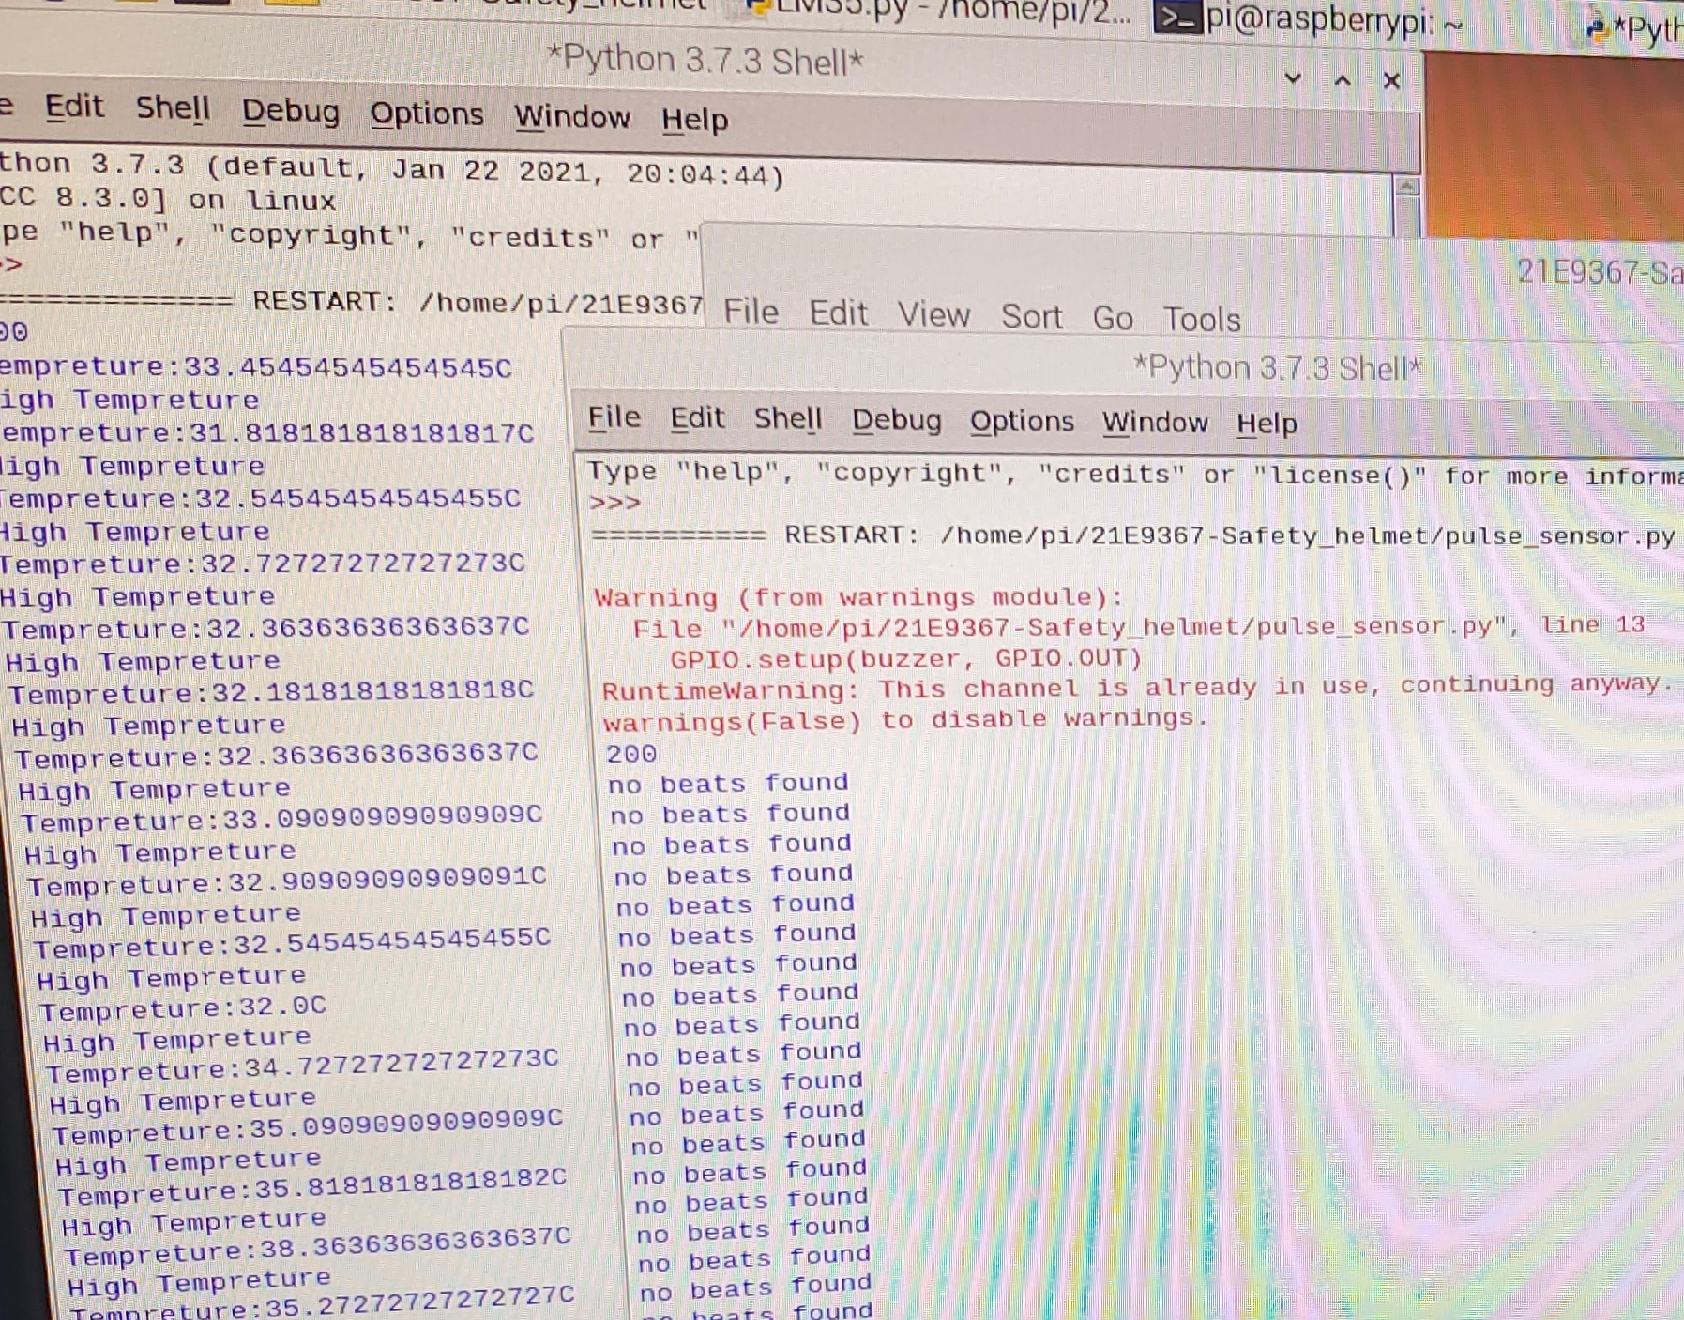
\includegraphics[width=18cm]{result.png}
    \caption{Result 1}
     
\end{figure}

\begin{figure}[htp]
    \includegraphics[width=18cm]{result 2 png.png}
    \caption{Result 2}

\end{figure}
\noindent Correspondingly , if the gas sensor  detects gas or smoke according to the given specific condition the buzzer will be on , or else the buzzer will be in the switch off condition.Further fig defines the data stored in cloud that is thinkspeak.

\begin{figure}[htp]
    \includegraphics[width=18cm]{2022-05-26.png}
    \caption{Result 3}
\end{figure}

\begin{figure}[htp]
    \includegraphics[width=18cm]{2022-05-26 (1).png}
    \caption{Result 4}
\end{figure}

\noindent \textbf{}

\noindent \textbf{}

\noindent \textbf{}

\noindent \textbf{}

\noindent \textbf{}

\noindent \textbf{ }
\newpage
\noindent
\noindent 
\noindent
\chapter{Advantage and Applications}
\section{ Advantages}


\noindent The advantages of the proposed system can be summarized as follow:

\begin{enumerate}
\item  Secure miners' safety in case of mining accidents that occurs due to environmental changes i.e., increase in temperature, leakage of dangerous gases, increase in heart rate of the worker.

\item  To communicate the coal miners inside the mines with the outside world.

\item  To keep surveillance on the conditions inside the mines and alert the miners in case of emergency crisis.

\item  Alerting the miners in case the helmet is take off.

\item  The system of smart helmet is utilized to avoid motor bikes accidents 

\item  To recognize them at real time in order to maintain safety of human being. 

\item  The IoT based-technology of smart helmet is a crucial issue, which improves safety of two-wheeler driving than, exist one.
\end{enumerate}

\noindent 

\section{Applications }

\noindent The proposed system can be employed at variety of applications such as:

\noindent 
\newline
\noindent
\newline
\noindent{1. Minning Industries:-}

\noindent The smart helmet for mining industry contains of numerous sensors which are static on the helmet. The sensors used are Gas Sensor, Temperature Sensor, Humidity Sensor, LDR for light intensity, and IR sensor to detect the miner wearing helmet or not.

\noindent 
\newline
\noindent
\newline
\noindent{2.Construction sites:-}

\noindent Construction professional is rising day by day as all need substructures to live and to work. Supplementary and more developments need to be completed on time with the safety of all the laborers working on site.

\noindent  IoT based smart construction helmet decrease construction locations accidence which can be minor or major causes consequence on the entire location as well as exertion of construction.

\noindent 

\noindent 
\newline
\noindent
\newline
\noindent{3. Disaster Prevention:-}

\noindent IoT based smart helmet decrease  accidence which can be minor or major causes consequence on the entire location.

\noindent 

\noindent 
\newline
\noindent
\newline
\noindent{4. Applied Science:-}

\noindent A smart helmet is a wearable device that has fascinated consideration in various fields, specifically in applied sciences, where wide-ranging studies have been showed in the past period. 

\noindent In this study, the contemporary status and trends of smart helmet research were systematically reviewed. 

\noindent 

\noindent 
\newline
\noindent
\newline
\noindent{5. Rescue Request:-}

\noindent In any kind of emergency conditions the worker can be rescued  immediately with the help of advanced features inbuilt in the safety helmet.

\noindent 

\noindent 
\newline
\noindent
\newline
\noindent{6. Police Services:-}
\noindent To toughen the fight against coronavirus, police and authorities across the globe have started using 'smart helmets' which take only a few seconds to precisely scan people's temperature. 

\noindent With speedy thermal screenings being measured as one of the options to recognize COVID-19 patients, the technology will be predominantly useful in resuming the economy and guaranteeing the safe drive of people in public places.

\noindent  Dubai police are using the helmets to screen people in compactly occupied areas, including sealed off localities. The smart helmets, used by the Dubai police, also has facial recognition abilities, license plate recognition and the capability to scan QR codes.

\noindent 

\noindent 
\newline
\noindent
\newline
\noindent{7.Motorbike Riders:-}

\noindent The bike element interconnects with the IoT Cloud and updates the satisfactory information. Originally, when the bike ignition is on, the system checks whether the operator wears the helmet. If he does not wear a helmet, a arrangement of warning messages are demonstrated within a time intermission and thus a fine amount is engendered and these details are stored on the Server via IOT. 

\noindent The fine minutiae are sent to the operator's enumerated mail Id via an computerized mailing system declaring the fine details of the defilement.

\noindent The operator is given a Login portal with a user Id and password during the registration which can be used to pay the fine. The operator will be given 15 days of time to pay the fine. On not compensable the fine, the fine amount will be doubled. After a month of time, the rider's license is canceled.

\noindent 

\noindent 
\newline
\noindent
\newline
\noindent{8. Medical Field:-}

\noindent In the medical field to improve the work productivity of medical staff and safeguard the safety of patients. In this application, a smart helmet worn by the medical staff was used to perceive body temperature and brain waves in emergency circumstances  A smart helmet was industrialized for medical staff to perceive the body temperature of a pedestrian in real time. It was used to avoid coronavirus by cautioning them through an alarm when realizing a high-temperature pedestrian

\noindent  
\newpage



\chapter{Conclusion and Future Scope}

\noindent \textbf{}

\noindent 

\noindent
\section{Conclusion}

\noindent The proposed methodology aids in both the prevention of workplace accidents and the preservation of society's cleanliness. The smart safety gadget is less expensive and more quickly connects  and transmits data to emergency department. Therefore, a smart helmet for detecting dangerous environmental conditions, monitoring workers heartrate and antique the information and the sensed data with the help of sensors to the control main unit for easy tracking and providing oxygen supplements to avoid the inhalation of hazardous gases is intended.

\noindent 
\section{Future Scope}

\noindent To avoid the range issues, we can attach a Signal/network Catcher. For better communication Walkie Talky can be added.\textbf{}

\noindent To date, there has been in-sufficient research on the security and privacy of data collected by smart helmets through sensors. It can be improved to maintain the privacy of data collection \& Small Fans.
\newpage


\chapter{References}

\noindent 

\begin{enumerate}
\item  ZigBee Alliance, ``Understanding ZigBee gateway'', ZigBee Document 095465r13, September 2010.

\item  Sobin, C. C. "A survey on architecture, protocols and challenges in IoT."~\textit{Wireless Personal Communications}~112, no. 3 (2020): 1383-1429.

\item  Malakahmad, A., Downe, A.G. and Fadzil, S.D.M., 2012, April. Application of occupational health and safety management system at sewage treatment plants. In 2012 IEEE Business, Engineering \& Industrial Applications Colloquium (BEIAC) (pp. 347-350). IEEE.

\item  Zhou, Mudi, Zhuli Fang, Bin Zhao, and Pengfei Li. "Safety Helmet Wearing Detection and Recognition Based on YOLOv4." In 2021 3rd International Academic Exchange Conference on Science and Technology Innovation (IAECST), pp. 798-802. IEEE, 2021.

\item  Gao, Yumin, Yan Liu, Daojin Nie, Ziming Huang, Bin Li, and Bing Qian. "An Efficient Safety Helmet Detection based on Attentional Mechanism." In 2021 7th International Symposium on System and Software Reliability (ISSSR), pp. 97-98. IEEE, 2021.

\item  Ren, Dacong, Tongsheng Sun, Cungui Yu, and Cheng Zhou. "Research on Safety Helmet Detection for Construction Site." In 2021 International Conference on Computer Information Science and Artificial Intelligence (CISAI), pp. 186-189. IEEE, 2021.

\item  Sharma, Susanta, Allumallu Veera Venkata Susmitha, Lan-Da Van, and Yu-Chee Tseng. "An Edge-Controlled Outdoor Autonomous UAV for Colorwise Safety Helmet Detection and Counting of Workers in 6Construction Sites." In 2021 IEEE 94th Vehicular Technology Conference (VTC2021-Fall), pp. 1-5. IEEE, 2021.

\item   Biradar, Priya, Priyanka Kolsure, Sujata Khodaskar, and Kishor B. Bhangale. "IoT based smart bracelet for women security."~\textit{Int. J. Res. Appl. Sci. Eng. Technol.(IJRASET)}~8, no. 11 (2020): 688-691.

\item  Sarraf, Rajan, Shalini Ojha, Damini Biraris, and Kishor B. Bhangale. "IoT based smart quality water management system."~\textit{International Journal}~Of Advance Scientific Research And Engineering Trends, 5, no. 3 (2020).

\item  Mapari, Rahul, Kishor Bhangale, Laukik Deshmukh, Prashant Gode, and Ankit Gaikwad. "Agriculture Protection from Animals Using Smart Scarecrow System." In~\textit{Soft Computing for Security Applications}, pp. 539-551. Springer, Singapore, 2022. 

\item  Asthana, Nitin, and Ridhima Bahl. "IoT device for sewage gas monitoring and alert system." In 2019 1st International Conference on Innovations in Information and Communication Technology (ICIICT), pp. 1-7. IEEE, 2019. 

\item  Freeman, Emmanuel, Daniel Ayitey Quaye, Israel Edem Agbehadji, and Richard C. Millham. "Nature-inspired search method for IoT-based water leakage location detection system." In 2019 International Conference on Mechatronics, Remote Sensing, Information Systems and Industrial Information Technologies (ICMRSISIIT), vol. 1, pp. 1-8. IEEE, 2020.

\item  Haswani, Navin G., and Pramod J. Deore. "Web-based realtime underground drainage or sewage monitoring system using wireless sensor networks." In 2018 Fourth International Conference on Computing Communication Control and Automation (ICCUBEA), pp. 1-5. IEEE, 2018.

\item  Tian, Jingwen, Hao Wu, and Meijuan Gao. "Measurement and control system of sewage treatment based on wireless sensor networks." In 2008 IEEE International Conference on Industrial Technology, pp. 1-4. IEEE, 2008.

\item  Malakahmad, Amirhossein, Alan Giffin Downe, and Siti Dhamina Muhamad Fadzil. "Application of occupational health and safety management system at sewage treatment plants." In 2012 IEEE Business, Engineering \& Industrial Applications Colloquium (BEIAC), pp. 347-350. IEEE, 2012.

\item  Priya, E., and A. Kumaran. "Automated detection of toxicity in the blood samples of dye factory workers." In 2015 International Conference on Computing and Communications Technologies (ICCCT), pp. 334-337. IEEE, 2015.

\item  Priyanka, Y. K., M. Gowtham, C. Yashashwini, C. B. Yashashwini, and H. C. Yashashwini. "Detection and Get Rid of Blockage in a Manhole Pipe Using IoT." In 2020 International Conference on Recent Trends on Electronics, Information, Communication \& Technology (RTEICT), pp. 204-207. IEEE, 2020.

\item  Umapathi, N., Sai Teja, and Sai Kiran. "Design and Implementation of Prevent Gas Poisoning from Sewage Workers using Arduino." In 2020 IEEE International Symposium on Sustainable Energy, Signal Processing and Cyber Security (iSSSC), pp. 1-4. IEEE, 2020.

\item  Pushpakumar, R., and S. Rajiv. "IOT based smart drainage worker safety system." International Journal of Innovative Technology and Exploring Engineering 8, no. 8 (2019): 1083-1086.

\item  Kumar, Sudhanshu, Saket Kumar, P. M. Tiwari, and Rajkumar Viral. "Smart Safety Monitoring System for Sewage workers with two way communication." In 2019 6th International Conference on Signal Processing and Integrated Networks (SPIN), pp. 617-622. IEEE, 2019.

\item  Kun Han ,Deep Learning-Based Workers Safety Helmet Wearing Detection on Construction Sites Using Multi-Scale Features Published in: IEEE Access ( Volume: 10) Page(s): 718 -- 729, 2021.

\item  Huang, Li, Qiaobo Fu, Meiling He, Du Jiang, and Zhiqiang Hao. "Detection algorithm of safety helmet wearing based on deep learning."~\textit{Concurrency and Computation: Practice and Experience}~33, no. 13 (2021): e6234.
\end{enumerate}

\noindent 

\noindent 

\noindent 
\newpage

\section{ Cost Estimation }
\begin{table}[ht]
    \centering
    \resizebox{\textwidth}{!}
    {
\begin{tabular}{|p{0.5in}|p{1.6in}|p{1.0in}|p{0.5in}|p{0.9in}|} \hline 
\textbf{Sr.no} & \textbf{Hardware Components} & \textbf{Version } & \textbf{Qty.} & \textbf{Total Cost } \\ \hline 
1. & Raspberry Pi 4 & Model B & 1 & 7,500/- \\ \hline 
2. & Monitor & - & 1 & 2,000/- \\ \hline 
3. & Keyboard & - & 1 & 541/- \\ \hline 
4. & Mouse & - & 1 & 449/- \\ \hline 
5. & HDMI to VGA converter & - & 1 & 500/- \\ \hline 
6. & Temperature Sensor & - & 1 & 85/- \\ \hline 
7. & Heartbeat Sensor  & - & 1 & 625/- \\ \hline 
8. & Smoke Sensor & - & 1 & 159/- \\ \hline 
9. & A-D converter & - & 1 & 600/- \\ \hline 
10. & HDMI cable  & - & 1 & 450/- \\ \hline 
11. & Buzzer & - & 1 & 40/- \\ \hline 
\multicolumn{4}{|p{1in}|}{Component Total Cost} & 12,949/- \\ \hline 
\multicolumn{4}{|p{1in}|}{Hiring Services Cost} & - \\ \hline 
\multicolumn{4}{|p{1in}|}{Total Project Cost (Components + Hiring)} & 12,949/- \\ \hline 
\end{tabular}
}
    \caption{Cost Estimation}
    \label{tab:my_label}
\end{table}


\appendix

\chapter{Project Outcomes}%This is just for showing, where it shows up, in my original, it says only Appendix here.
\newpage
\section{Plagiarism Report For Research Paper}
\begin{figure}[htp]
    \includegraphics[width=15cm]{2022-05-24-min.png}
\end{figure}

\newpage
\section{Plagiarism Report}
\begin{figure}[htp]
    \includegraphics[width=15cm]{2022-05-16 (5)-min.png}
\end{figure}

\newpage
\section {Copyright Certificate and Work Uploaded}
\begin{figure}[htp]
    \includegraphics[width=15cm]{2022-05-16 (7).png}
\end{figure}
\begin{figure}[htp]
    \includegraphics[width=18cm]{2022-05-16 (8).png}
\end{figure}
\newpage
\section{Publication Certificates}
\begin{figure}[htp]
    \includegraphics[width=18cm]{2022-06-03.png}
\end{figure}
\begin{figure}[htp]
    \includegraphics[width=18cm]{2022-06-03 (2).png}
\end{figure}
\begin{figure}[htp]
    \includegraphics[width=18cm]{2022-06-03 (1).png}
\end{figure}
\newpage
\newpage
\section{UGCON Certificate}
\begin{figure}[htp]
    \includegraphics[width=18cm]{2022-06-03 (3).png}
\end{figure}
\begin{figure}[htp]
    \includegraphics[width=18cm]{2022-06-03 (4).png}
\end{figure}
\begin{figure}[htp]
    \includegraphics[width=18cm]{2022-06-03 (5).png}
\end{figure}

\end{document}